%!TEX root = da-screen.tex

In this chapter we will prove Ramsey's theorem, which is a mathematical statement with numerous applications. This chapter is pure combinatorics; we will not discuss distributed algorithms at all. In Chapter~\ref{ch:ramsey-app} we will then see how to apply Ramsey's theorem to prove negative results related to distributed algorithms.


\section{Monochromatic Subsets}

Let $Y$ be a finite set. We say that $X$ is a \emph{$k$-subset} of $Y$ if $X \subseteq Y$ and $|X| = k$. We use the notation
\[
    Y^{(k)} = \{ X \subseteq Y : |X| = k \}
\]
for the collection of all $k$-subsets of $Y$.

A \emph{$c$-labelling} of $Y^{(k)}$ is an arbitrary function
\[
    f \colon Y^{(k)} \to \{1,2,\dotsc,c\}.
\]
Fix some $Y$, $k$, $c$, and $f$, where $f$ is a $c$-labelling of $Y^{(k)}$. We say that
\begin{enumerate}
    \item $X \subseteq Y$ is \emph{monochromatic in $f$} if $f(A) = f(B)$ for all $A, B \in X^{(k)}$,
    \item $X \subseteq Y$ is \emph{almost monochromatic in $f$} if $f(A) = f(B)$ for all $A, B \in X^{(k)}$ with $\min(A) = \min(B)$.
\end{enumerate}
See Figure~\ref{fig:monochromatic} for examples. Monochromatic subsets are a central concept in Ramsey theory, while almost monochromatic subsets are a technical definition that we will use in the proof.

\begin{figure}
    \centering
    \begin{tabular}{c@{\hspace{5ex}}c}
        \toprule
        \multicolumn{2}{@{}c@{}}{$f \colon Y^{(2)} \to \{1,2,3\}$} \\
        \midrule
        $\{1,2\} \mapsto 1$ & $\{2,4\} \mapsto 1$ \\ 
        $\{1,3\} \mapsto 1$ & $\{2,5\} \mapsto 2$ \\
        $\{1,4\} \mapsto 2$ & $\{3,4\} \mapsto 3$ \\
        $\{1,5\} \mapsto 1$ & $\{3,5\} \mapsto 3$ \\
        $\{2,3\} \mapsto 2$ & $\{4,5\} \mapsto 3$ \\
        \bottomrule
    \end{tabular}
    \caption{In this example, $Y = \{1,2,3,4,5\}$. Function $f$ is a $3$-labelling of $Y^{(2)}$. Set $\{1,2,3,5\}$ is almost monochromatic but not monochromatic in $f$. Set $\{3,4,5\}$ is both almost monochromatic and monochromatic in $f$.}\label{fig:monochromatic}
\end{figure}


\section{Ramsey Numbers}

For all positive integers $c$, $n$, and $k$, we define the numbers $R_c(n;k)$ and $\bar{R}_c(n;k)$ as follows.
\begin{enumerate}
    \item $R_c(n;k)$ is the smallest natural number $N$ such that the following holds: for any set $Y$ with at least $N$ elements, and for any $c$-labelling $f$ of $Y^{(k)}$, there is an $n$-subset of $Y$ that is monochromatic in $f$. If no such $N$ exists, $R_c(n;k) = \infty$.
    \item $\bar{R}_c(n;k)$ is the smallest natural number $N$ such that the following holds: for any set $Y$ with at least $N$ elements, and for any $c$-labelling $f$ of $Y^{(k)}$, there is an $n$-subset of $Y$ that is almost monochromatic in $f$. If no such $N$ exists, $\bar{R}_c(n;k) = \infty$.
\end{enumerate}
Numbers $R_c(n;k)$ are called \emph{Ramsey numbers}, and Ramsey's theorem shows that they are always finite.

\begin{theorem}[Ramsey's theorem]\label{thm:ramsey}
    Numbers $R_c(n;k)$ are finite for all positive integers $c$, $n$, and $k$.
\end{theorem}

We will prove Theorem~\ref{thm:ramsey} in Section~\ref{ssec:ramsey-proof}; let us first have a look at an application.


\section{An Application}

In the case of $k = 2$, Ramsey's theorem can be used to derive various graph-theoretic results. As a simple application, we can use Ramsey's theorem to prove that sufficiently large graphs necessarily contain large cliques or large independent sets.

Let $G = (V,E)$ be a graph. Recall that an \emph{independent set} is a subset $X \subseteq V$ such that $\{u,v\} \notin E$ for all $\{u, v\} \in X^{(2)}$. A complementary concept is a \emph{clique}: it is a subset $X \subseteq V$ such that $\{u,v\} \in E$ for all $\{u, v\} \in X^{(2)}$.

\begin{lemma}
    For any natural number $n$ there is a natural number $N$ such that the following holds:
    if $G = (V,E)$ is a graph with at least $N$ nodes,
    then $G$ contains a clique with $n$ nodes or an independent set with $n$ nodes.
\end{lemma}
\begin{proof}
    Choose an integer $N \ge R_2(n;2)$; by Theorem~\ref{thm:ramsey}, such an $N$ exists.
    
    Now if $G = (V,E)$ is any graph with at least $N$ nodes, we can define a $2$-labelling $f$ of $V^{(2)}$ as follows:
    \[
        f(\{u,v\}) = \begin{cases}
            1 & \text{if } \{u,v\} \in E, \\
            2 & \text{if } \{u,v\} \notin E.
        \end{cases}
    \]
    By the definition of Ramsey numbers, if $|V| \ge N$, there is an $n$-subset $X \subseteq V$ that is monochromatic in $f$.
    If $X \subseteq V$ is monochromatic, we have one of the following cases:
    \begin{enumerate}
        \item we have $f(\{u,v\}) = 1$ for all $\{u,v\} \in X^{(2)}$; therefore $X$ is a clique,
        \item we have $f(\{u,v\}) = 2$ for all $\{u,v\} \in X^{(2)}$; therefore $X$ is an independent set. \qedhere
    \end{enumerate}
\end{proof}


\section{Proof}\label{ssec:ramsey-proof}

Let us now prove Theorem~\ref{thm:ramsey}. Throughout this section, let $c$ be fixed. We will show that $R_c(n;k)$ is finite for all $n$ and $k$. The proof outline is as follows:
\begin{enumerate}
    \item Lemma~\ref{lem:pigeonhole}: $R_c(n;1)$ is finite for all $n$.
    \item Corollary~\ref{cor:RtoR}: if $R_c(n;k-1)$ is finite for all $n$, then $R_c(n;k)$ is finite for all $n$.
    
        Here we will use the following auxiliary results:
        \begin{enumerate}[label=(\roman*)]
            \item Lemma~\ref{lem:RtoG}\mydash if $R_c(n;k-1)$ is finite for all $n$, then $\bar{R}_c(n;k)$ is finite for all $n$.
            \item Lemma~\ref{lem:GtoR}\mydash if $\bar{R}_c(n;k)$ is finite for all $n$, then $R_c(n;k)$ is finite for all $n$.
        \end{enumerate}
    \item Now by induction on $k$, it follows that $R_c(n;k)$ is finite for all $n$ and $k$.
\end{enumerate}

The base case of $k = 1$ is, in essence, equal to the familiar pigeonhole principle.

\begin{lemma}\label{lem:pigeonhole}
    Ramsey number $R_c(n;1)$ is finite for all $n$.
\end{lemma}
\begin{proof}
    Let $N = c(n-1)+1$. We can use the pigeonhole principle to show that $R_c(n;1) \le N$.
    
    Let $Y$ be a set with at least $N$ elements, and let $f$ be a $c$-labelling of $Y^{(1)}$.
    In essence, we have $c$ boxes, labelled with $\{1,2,\dotsc,c\}$, and function $f$ places each element of $Y$ into one of these boxes.
    As there are $N$ elements, there is a box that contains at least
    \[
        \lceil N/c \rceil = n
    \]
    elements. These elements form a monochromatic subset.
\end{proof}

Let us now study the case of $k > 1$. We begin with a technical lemma.

\begin{lemma}\label{lem:RtoGpart}
    Let $n$ and $k$ be integers, $n > k > 1$.
    If $M = \bar{R}_c(n-1;k)$ and $R_c(M;k-1)$ are finite, then $\bar{R}_c(n;k)$ is finite.
\end{lemma}
\begin{proof}
    Define
    \[
        N = 1 + R_c(M;k-1).
    \]
    We will prove that $\bar{R}_c(n;k) \le N$.
    
    Let $Y$ be a set with $N$ elements; w.l.o.g., we can assume that $Y = \{1,2,\dotsc,N\}$. Let $f$ be any $c$-labelling of $Y^{(k)}$. We need to show that there is an almost monochromatic $n$-subset $W \subseteq Y$.
    
    To this end, let $Y_2 = \{2,3,\dotsc,N\}$, and define a $c$-labelling $f_2$ of $Y_2^{(k-1)}$ as follows; see Figure~\ref{fig:RtoGpart} for an illustration:
    \[
        f_2(A) = f(\{1\} \cup A) \ \text{ for each } A \in Y_2^{(k-1)}.
    \]
    Now $f_2$ is a $c$-labelling of $Y_2^{(k-1)}$, and $Y_2$ contains
    \[
        N - 1 = R_c(M;k-\nobreak 1)
    \]    
    elements. Hence, by the definition of Ramsey numbers, there is an $M$-subset $X_2 \subseteq Y_2$ that is monochromatic in $f_2$.

\begin{figure}
    \centering
    \includegraphics[page=\PRtoGPart]{figs.pdf}
    \caption{The proof of Lemma~\ref{lem:RtoGpart}, for the case of $c = 2$, $k = 3$, and $n = 5$, assuming completely fictional values $M = 5$ and $N = 7$.}\label{fig:RtoGpart}
\end{figure}
    
    Function $f$ is a $c$-labelling of $Y^{(k)}$, and $X_2 \subseteq Y$. Hence by restriction $f$ defines a $c$-labelling of $X_2^{(k)}$. Set $X_2$ contains $M = \bar{R}_c(n-\nobreak 1;k)$ elements. Therefore there is an $(n-\nobreak 1)$-subset $W_2 \subseteq X_2$ that is almost monochromatic in $f$.
    
    To conclude the proof, let $W = \{1\} \cup W_2$. By construction, $W$ contains $n$ elements. Moreover, $W$ is almost monochromatic in $f$. To see this, assume that $A,B \subseteq W$ are $k$-subsets such that $\min(A) = \min(B)$. We need to show that $f(A) = f(B)$. There are two cases:
    \begin{enumerate}
        \item We have $\min(A) = \min(B) = 1$. Let $A_2 = A \setminus \{1\}$ and $B_2 = B \setminus \{1\}$. Now $A_2$ and $B_2$ are $(k-1)$-subsets of $X_2$. Set $X_2$ was monochromatic in $f_2$, and hence $f(A) = f_2(A_2) = f_2(B_2) = f(B)$.
        \item Otherwise $1 \notin A$ and $1 \notin B$. Now $A$ and $B$ are $k$-subsets of $W_2$. Set $W_2$ was almost monochromatic in $f$, and we have $\min(A) = \min(B)$, which implies $f(A) = f(B)$. \qedhere
    \end{enumerate}
\end{proof}

\begin{lemma}\label{lem:RtoG}
    Let $k > 1$ be an integer.
    If $R_c(n;k-1)$ is finite for all $n$, then $\bar{R}_c(n;k)$ is finite for all $n$.
\end{lemma}
\begin{proof}
    The proof is by induction on $n$.
    
    The base case of $n \le k$ is trivial: a set with $n$ elements has at most one subset with $k$ elements, and hence it is almost monochromatic and monochromatic.
    
    Now let $n > k$. Inductively assume that $\bar{R}_c(n-1;k)$ is finite. Recall that in the statement of this lemma, we assumed that $R_c(M;k-1)$ is finite for any $M$; in particular, it is finite for $M = \bar{R}_c(n-1;k)$. Hence we can apply Lemma~\ref{lem:RtoGpart}, which implies that $\bar{R}_c(n;k)$ is finite.
\end{proof}

\begin{lemma}\label{lem:GtoR}
    Let $k > 1$ be an integer.
    If $\bar{R}_c(n;k)$ is finite for all $n$, then $R_c(n;k)$ is finite for all $n$.
\end{lemma}
\begin{proof}
    Let $M = R_c(n;1)$. By Lemma~\ref{lem:pigeonhole}, $M$ is finite. By assumption, $\bar{R}_c(M;k)$ is also finite. We will show that
    \[
        R_c(n;k) \le \bar{R}_c(M;k).
    \]
    
    Let $Y$ be a set with $N = \bar{R}_c(M;k)$ elements, and let $f$ be any $c$-labelling of $Y^{(k)}$. We need to show that there is a monochromatic $n$-subset $W \subseteq Y$.
    
    By definition, there is an almost monochromatic $M$-subset $X \subseteq Y$. Hence we can define a $c$-labelling $g$ of $X^{(1)}$ such that
    \[
        g( \{ \min(A) \} ) = f(A)
    \]
    for each $k$-subset $A \subseteq X$; see Figure~\ref{fig:GtoR}. As $X$ is a subset with $M = R_c(n;1)$ elements, we can find an $n$-subset $W \subseteq X$ that is monochromatic in $g$.

\begin{figure}
    \centering
    \begin{tabular}{c@{\hspace{5ex}}c}
        \toprule
        $f$ & $g$ \\
        \midrule
        $\{1,2\} \mapsto 1$ & $\{1\} \mapsto 1$ \\ 
        $\{1,3\} \mapsto 1$ & \\
        $\{1,4\} \mapsto 1$ & \\
        \midrule
        $\{2,3\} \mapsto 3$ & $\{2\} \mapsto 3$ \\
        $\{2,4\} \mapsto 3$ & \\
        \midrule
        $\{3,4\} \mapsto 2$ & $\{3\} \mapsto 2$ \\
        \midrule
                            & $\{4\} \mapsto 1$ \\
        \bottomrule
    \end{tabular}
    \caption{The proof of Lemma~\ref{lem:GtoR}. In this example, $c=3$, $k=2$, and $X = \{1,2,3,4\}$ is almost monochromatic in $f$. We define a $c$-labelling $g$ of $X^{(1)}$ such that $g( \{ \min(A) \} ) = f(A)$ for all $A \in X^{(2)}$. Note that the choice of $g({4})$ is arbitrary.}\label{fig:GtoR}
\end{figure}
    
    Now we claim that $W$ is also monochromatic in $f$. To see this, let $A$ and $B$ be $k$-subsets of $W$. Let $x = \min(A)$ and $y = \min(B)$. We have $x, y \in W$ and
    \[
        f(A) = g(\{x\}) = g(\{y\}) = f(B). \qedhere
    \]
\end{proof}

Lemmas \ref{lem:RtoG} and \ref{lem:GtoR} have the following corollary.

\begin{corollary}\label{cor:RtoR}
    Let $k > 1$ be an integer.
    If $R_c(n;k-1)$ is finite for all $n$, then $R_c(n;k)$ is finite for all $n$.
\end{corollary}

Now Ramsey's theorem follows by induction on $k$: the base case is Lemma~\ref{lem:pigeonhole}, and the inductive step is Corollary~\ref{cor:RtoR}.


\section{Exercises}

\begin{ex}
    Prove that $R_c(n;1) = c\cdot(n-1)+1$.
    
    \hint{The proof of Lemma~\ref{lem:pigeonhole} shows that \[R_c(n;1) \le c\cdot(n-1)+1.\] You need to show that \[R_c(n;1) > c\cdot(n-1).\]}
\end{ex}

\begin{ex}
    Prove that $R_2(3;2) \ge 6$.

    \hint{Prove that $R_2(3;2) > 5$. That is, show that there is a $2$-labelling of $2$-subsets of a base set of size $5$ such that there is no monocromatic subset of size $3$.}
\end{ex}

\begin{ex}
    Prove that $R_2(3;2) \le 6$. Together with the previous exercise, this will show that $R_2(3;2) = 6$.
\end{ex}

\begin{ex}
    Prove a non-trivial lower bound on $R_2(4;2)$. For example, show that $R_2(4;2) \ge 10$.
\end{ex}

\begin{ex}
    Prove some concrete upper bound on $R_2(4;2)$. For example, show that $R_2(4;2) \le 100$.
\end{ex}

\begin{exs}
    Find the exact value of $R_2(4;2)$.
\end{exs}


\section{Bibliographic Notes}

Ramsey's theorem dates back to 1930s~\cite{ramsey30problem}; our proof follows Ne{\v s}et{\v r}il \cite{nesetril95ramsey}, and the notation is from Radziszowski~\cite{radziszowski11ramsey}.
